%
% General structure for the revdetua class:
%
\documentclass[longpaper, english, final, times]{revdetua}
%
% Valid options are:
%
%   longpaper --------- \part and \tableofcontents defined
%   shortpaper -------- \part and \tableofcontents not defined (default)
%
%   english ----------- main language is English (default)
%   portugues --------- main language is Portuguese
%
%   draft ------------- draft version
%   final ------------- final version (default)
%
%   times ------------- use times (postscript) fonts for text
%
%   mirror ------------ prints a mirror image of the paper (with dvips)
%
%   visiblelabels ----- \SL, \SN, \SP, \EL, \EN, etc. defined
%   invisiblelabels --- \SL, \SN, \SP, \EL, \EN, etc. not defined (default)
%
% Note: the final version should use the times fonts
% Note: the really final version should also use the mirror option
%

\usepackage{amsmath, amssymb}
\usepackage{enumitem}
\usepackage{booktabs} % To thicken table lines
%\usepackage{longtable}
\usepackage{arydshln}
\usepackage{graphicx}
\usepackage{dblfloatfix} % fix for table placement


%% ALGORITHM 1 PROCEEDURES-----------------------------------------
%\usepackage{algorithm}
%%\usepackage[algo2e]{algorithm2e} 
%\usepackage{arevmath}     % For math symbols
%\usepackage[noend]{algpseudocode}

%% ALGORITHM 2 FUNCTIONS-----------------------------------------
\usepackage{xcolor}
\usepackage[linesnumbered,ruled,vlined]{algorithm2e}
% set comment color to blue
\newcommand\mycommfont[1]{\footnotesize\ttfamily\textcolor{blue}{#1}}
\SetCommentSty{mycommfont}

% drawing trees
\usepackage{tikz}
\usetikzlibrary{trees}

\usepackage{tikz}
\usetikzlibrary{arrows, positioning, automata}

\begin{document}
	
	%\Header{Volume}{Number}{Month}{Year}{InitialPage}
	% Note: the month must be in Portuguese
	
	\title{Probabilistic Counters}
	\author{ABLORDEPPEY Prosper} % or \author{... \and ...}
	\maketitle
	
	\begin{abstract}% Note: in English
		In this project, the goal is to count the number of occurrences of letters in text files and, for instance, identify the most common ones. Three types of counters were analyzed. The \textit{Exact Counter}; which provides the exact count or frequency of each letter present in the text, the \textit{Fixed Probability Counter}, which approximates the frequency or number of counts of each letter in the text using a fixed probability value of $\frac{1}{2}$. The last counting method considered, being the \textit{Decreasing Probability Counter} approximates the count of each letter in the text with each future encounter of the letter having a decreased probability of being counter, with probability $\left(\frac{1}{\sqrt{2}^k}\right)$ where $k$ is the number of occurrence of the letter of interest.
	\end{abstract}
	
%	\begin{resumo}% Note: in Portuguese
%		...
%	\end{resumo}
	
	\begin{keywords}% Note: in English (optional)
		\begin{enumerate}
			\item Let $k_n$ denote the counter value of a given counter for the $n'th$ occurrence of a letter in the text stream.
			\item Let $\mathbb{E}[k_n]$ denote the Expected Counter Value for the $n'th$ occurrence.
			\item From a Counter Value $k_n$, we denote an estimate of the actual/exact number of occurrence for $n$ as $\hat{n}$.
		\end{enumerate}
	\end{keywords}
	
%	\begin{palavraschave}% Note: in Portuguese (optional)
%		...
%	\end{palavraschave}

	\section{Basic Derivations}
		Let $X_i$ be a random variable modeling the $i'th$ increment with binary states $S=\{0,1\}$ where $X_i=0$ is the event of not increasing the counter value and $X_i=1$ be the event of increasing the counter value.\\
		 
		Again, let $p$ and $q$ be the probability of increasing and not increasing the counter value respectively. Thus
		\begin{align*}
			\mathbb{P}(X_i=1)&=p \\
			\mathbb{P}(X_i=0)&=1-p=q
		\end{align*}
		\begin{align*}
			\intertext{Moments}
			\mathbb{E}[X] &= \sum_{i\in S}x_i\cdot \mathbb{P}(x=i) \tag{1}\\
			&=0\cdot (1-p)+1\cdot p=p \\
			\therefore \mathbb{E}[X] &= p \\
			\mathbb{E}[X^2] &= \sum_{i\in S}x_i^2\cdot \mathbb{P}(x=i)\\
			&=0^2\cdot (1-p)+1^2\cdot p=p \\
			\therefore \mathbb{E}[X^2] &= p \\
		\end{align*}
		\begin{align*}
			\intertext{For the $n'th$ occurrence, the counter value is expressed as}
			k_n &= \sum_{i=1}^{n}X_i \\
			\mathbb{E}[k_n]&=\mathbb{E}\left[\sum_{i=1}^{n}X_i\right]\\
			&=\sum_{i=1}^{n}\mathbb{E}[X] \\
			&=n\cdot \mathbb{E}[X] \\
			&=n\cdot p
		\end{align*}
		\begin{align*}
			\sigma^2[k_n]&=\sum_{i=1}^{n}\sigma^2\left[X\right]\\
			&=\sum_{i=1}^{n}\left[\mathbb{E}[X^2]-\mathbb{E}[X]^2\right] \\
			&=\sum_{i=1}^{n}\left[p-p^2\right]\\
			&=n(p-p^2) \\
			&=n\cdot p\cdot=(1-p)=n\cdot p\cdot q
		\end{align*}
		It has been shown from the above that, for the $n'th$ occurrence of a given letter, the expected counter value, variance and standard deviation are expressed respectively as;
		\begin{align}
			\mathbb{E}[k_n] = n\cdot p \label{equation1}\\
			\sigma^2[k_n] = n\cdot p\cdot q \label{equation2}\\
			\sigma[k_n] = \sqrt{n\cdot p\cdot q} \label{equation3}
		\end{align}
		
			
	\section{Outline Of Implementation}
		
	 	
	\section{EXACT COUNTER}
		This counter could be considered as a fixed probability counter, where the probability of increasing the counter value for a given new encounter of a letter is $p=1$. Anytime a new letter is observed from the text stream, the counter value get increased. Thus, $q=0$.
		Hence, the expected value, variance and standard deviation of the counter values is given as
		\begin{align*}
			\mathbb{E}[k_n] &= n\cdot p\\
			&=n\cdot 1=n \\
			\sigma^2[k_n] &= n\cdot p\cdot q\\
			&=n\cdot 1 \cdot 0=0 \\
			\sigma[k_n] &= \sqrt{n\cdot p\cdot q}\\
			&=\sqrt{n\cdot 1\cdot 0}=0
		\end{align*}
		
		The Table (\ref{table:exactCounterExpectedEstimate}) below presents the expected counter value for a given occurrence $n$ of a particular letter in a given text stream. The estimated occurrence from the $(k_n)$ counter values given as $(\widehat{n})$ is an identity relation.\\
		More formally,
		\begin{align*}
			\widehat{n} &= \mathbb{E}[k_n]
		\end{align*}
		
		Although such a counter will report the accurate/exact number of occurrence of each letter in the text stream, for large text streams, this becomes a problem as it occupies a lot of memory, hence, expensive. This motivates the notion of analyzing approximate counters with fixed probability and decreasing probabilities.
		\begin{table}[ht!]
			\begin{center}
				\label{table:exactCounterExpectedEstimate}
				\caption{Exact Counter Estimates}	
				{\def\arraystretch{2}%
					\begin{tabular}{l|l|c|c}
						\toprule
						Occurrence $(n)$ & Expected Value& $\mathbb{E}[k_n]$ & $\hat{n}$\\
						\hline
						1 & 1 & 1 & 1\\
						3 & $1+1+1$&3 & 3\\
						13 & $\mathbb{E}[k_{11}]+1+1$&13& 13\\
						27 & $\mathbb{E}[k_{25}]+1+1$&27 & 27\\
						51 & $\mathbb{E}[k_{49}]+1+1$&51 & 51\\
						\bottomrule
					\end{tabular}
				}
			\end{center}
		\end{table}
	 	
	 	\begin{figure}[ht!]
	 		\centering
	 		\caption{Exact Expected Counter Estimates}
	 		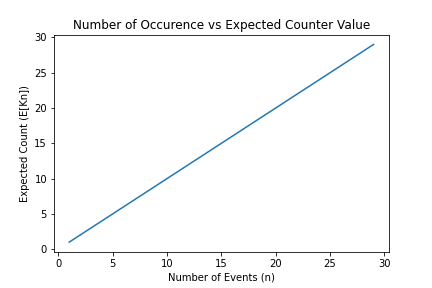
\includegraphics[width=260px, height=200px]{imgs/exact.png}		
	 	\end{figure}
		
				
	\section{FIXED PROBABILITY COUNTER}
		With this counter, the probability of increasing and decreasing the counter are equal. Thus $p=q=\frac{1}{2}$.
		Inferring from Equations (\ref{equation1}), (\ref{equation2}) and (\ref{equation3});
		\begin{align*}
			\mathbb{E}[k_n] &= n\cdot p\\
			&=n\cdot \frac{1}{2}=\frac{n}{2} \\
			\sigma^2[k_n] &= n\cdot p\cdot q\\
			&=n\cdot \frac{1}{2} \cdot \frac{1}{2}=\frac{n}{4} \\
			\sigma[k_n] &= \sqrt{n\cdot p\cdot q}\\
			&=\sqrt{n\cdot \frac{1}{2}\cdot \frac{1}{2}}=\frac{\sqrt{n}}{2}
		\end{align*}
	
		An expression for $\widehat{n}$ from the counter value $k_n$ for this counter is expressed as
		\begin{align*}
			\widehat{n}&= 2\cdot \mathbb{E}[k_n]
		\end{align*}
		This estimate relation evaluates to the actual number of occurrence $(n)$. The memory allocation for this counter is lesser than that of the exact counter by half $(\frac{1}{2})$.
	
		\begin{table}[!ht!]
			\begin{center}
				\label{table:fixedProbCounterExpectedEstimate}
				\caption{Fixed Probability Counter Estimates $\left(p=\frac{1}{2}\right)$}	
				{\def\arraystretch{2}%
					\begin{tabular}{l|l|c|c}
						\toprule
						Occurrence $(n)$ & Expected Value& $\mathbb{E}[k_n]$ & $\widehat{n}$\\
						\hline
						2&$\frac{1}{2}+\frac{1}{2}$&1&1\\
						4&$\mathbb{E}[k_{2}]+\frac{1}{2}+\frac{1}{2}$&2&4\\
						6& $\mathbb{E}[k_{4}]+\frac{1}{2}+\frac{1}{2}$&3&6\\
						28 & $\mathbb{E}[k_{26}]+\frac{1}{2}+\frac{1}{2}$&14&28\\
						50 & $\mathbb{E}[k_{48}]+\frac{1}{2}+\frac{1}{2}$&25&50\\
						\bottomrule
					\end{tabular}
				}
			\end{center}
		\end{table}
	
		\begin{figure}[ht!]
			\centering
			\caption{Fixed Prob Expected Counter Estimates}
			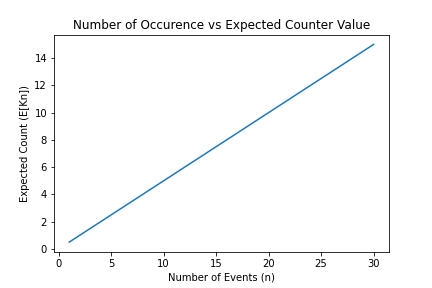
\includegraphics[width=260px, height=200px]{imgs/fixed.png}		
		\end{figure}	
	
	\section{DECREASING PROBABILITY COUNTER}
	
		% Define styles for bags and leafs
		\tikzstyle{bag} = [text width=4em, text centered]
		\tikzstyle{end} = [circle]
		
		\begin{figure}
			\begin{center}
				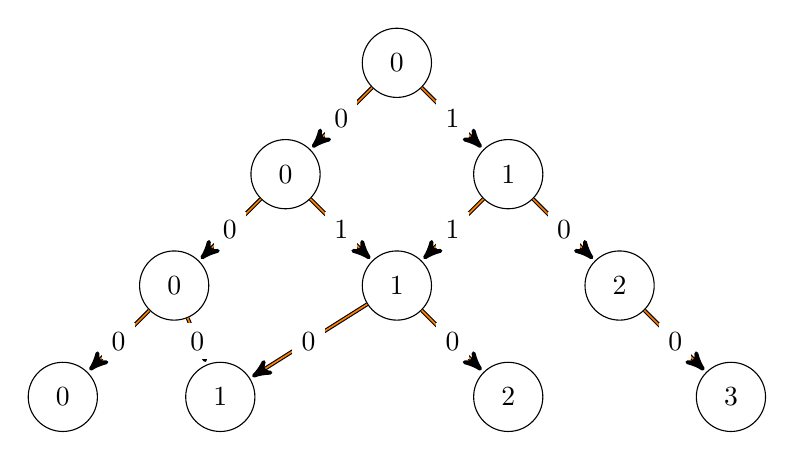
\begin{tikzpicture}[>=stealth',shorten >=1pt,node distance=2cm,on grid,initial/.style={}]
					\node[state] (T1) {$0$};
					\node[state] (T2) [below left =of T1] {$0$};
					\node[state] (T3) [below right  =of T1] {$1$};
					\node[state] (T4) [below left =of T2] {$0$};
					\node[state] (T5) [below right  =of T2] {$1$};
					\node[state] (T6) [below right =of T3] {$2$};
					\node[state] (T7) [below left =of T4] {$0$};
					\node[state] (T8) [right =of T7] {$1$};
					\node[state] (T9) [below right =of T5] {$2$};
					\node[state] (T10) [below right =of T6] {$3$};
					
					\tikzset{mystyle/.style={->,double=orange}}
					\tikzset{every node/.style={fill=white}}
					
					\path (T1) edge [mystyle] node {$0$} (T2);
					\path (T1) edge [mystyle] node {$1$} (T3);
					
					\path (T2) edge [mystyle] node {$0$} (T4);
					\path (T2) edge [mystyle] node {$1$} (T5);
					\path (T3) edge [mystyle] node {$1$} (T5);
					\path (T3) edge [mystyle] node {$0$} (T6);
					
					\path (T4) edge [mystyle] node {$0$} (T7);
					\path (T4) edge [mystyle] node {$0$} (T8);
					\path (T5) edge [mystyle] node {$0$} (T8);
					\path (T5) edge [mystyle] node {$0$} (T9);
					\path (T6) edge [mystyle] node {$0$} (T10);
%					\path (T3) edge [mystyle] node {$1$} (T7);
				\end{tikzpicture}
				\caption{Corrected Acyclic Graph}
			\end{center}
		\end{figure}
		
		
		\begin{figure}
			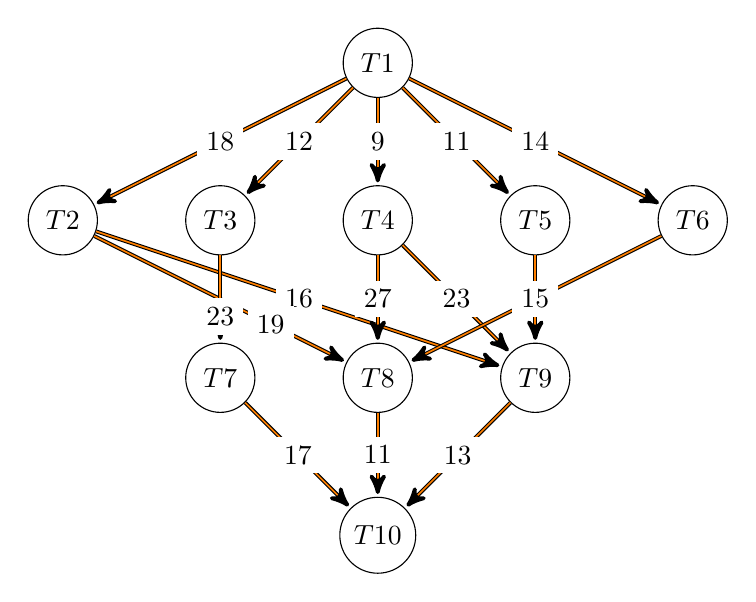
\begin{tikzpicture}[>=stealth',shorten >=1pt,node distance=2cm,on grid,initial/.style={}]
				\node[state] (T1) {$T1$};
				\node[state] (T4) [below =of T1] {$T4$};
				\node[state] (T3) [left  =of T4] {$T3$};
				\node[state] (T2) [left  =of T3] {$T2$};
				\node[state] (T5) [right =of T4] {$T5$};
				\node[state] (T6) [right =of T5] {$T6$};
				\node[state] (T8) [below =of T4] {$T8$};
				\node[state] (T7) [left  =of T8] {$T7$};
				\node[state] (T9) [right =of T8] {$T9$};
				\node[state] (T10) [below =of T8] {$T10$};
				
				\tikzset{mystyle/.style={->,double=orange}}
				\tikzset{every node/.style={fill=white}}
				\path (T1) edge [mystyle] node {$18$} (T2);
				\path (T1) edge [mystyle] node {$12$} (T3);
				\path (T1) edge [mystyle] node {$9$}  (T4);
				\path (T1) edge [mystyle] node {$11$} (T5);
				\path (T1) edge [mystyle] node {$14$} (T6);
%				\path (T2) edge [mystyle] node {$19$} (T8);
				\path (T2) edge [mystyle] node {$16$} (T9);
%				\path (T3) edge [mystyle] node {$23$} (T7);
				
				\path (T2) edge [mystyle] node[pos=0.7] {$19$} (T8);
				\path (T3) edge [mystyle] node[pos=0.7] {$23$} (T7);
				\path (T4) edge [mystyle] node {$27$} (T8);
				\path (T4) edge [mystyle] node {$23$} (T9);
				\path (T5) edge [mystyle] node {$13$} (T9);
				\path (T6) edge [mystyle] node {$15$} (T8);
				\path (T7) edge [mystyle] node {$17$} (T10);
				\path (T8) edge [mystyle] node {$11$} (T10);
				\path (T9) edge [mystyle] node {$13$} (T10);
			\end{tikzpicture}
			\caption{Corrected Acyclic Graph}
		\end{figure}
		
		\begin{tikzpicture}[level distance=1.3cm,
			level 1/.style={sibling distance=4cm},
			level 2/.style={sibling distance=1.6cm}]
			level 3/.style={sibling distance=0.1cm}]
%			\tikzstyle{every node}=[circle,draw]
			
%			\node (Root) [red] {0}
			\node (Root) {0}
			
			child {
%				node{0}
				node[] {0}
				edge from parent[black]
%				node[above] {3}
%				node[below]  {$\frac{4}{9}$}
				child{
					node {0}
					edge from parent[black]
					child {
						node[black] {0}
						edge from parent[black]
					}
					child { 
						node {1} 
					} 
				}
				child { 
					node {1}
					child { 
						node {1} 
					}
					child { 
						node {2} 
					}
				}
			}
			child {
				node {1} 
				child { 
					node {2}
					child { 
						node {3} 
					}
					child { 
						node {2} 
					}
				}
				child { 
					node {1}
					child { 
						node {2} 
					}
					child { 
						node {1} 
					}
				}
			};
		\end{tikzpicture}
	
		The probability of increasing the counter value for a given occurrence in this case is given as $p=\frac{1}{\sqrt{2}^{k_n}}$. Hence, $q=1-\frac{1}{\sqrt{2}^{k_n}}$.
		Inferring from Equations (\ref{equation1}), (\ref{equation2}) and (\ref{equation3});
		\begin{align*}
			\mathbb{E}[k_n] &= n\cdot p\\
			&=n\cdot \frac{1}{\sqrt{2}^{k_n}}=\frac{n}{\sqrt{2}^{k_n}} \\
			\sigma^2[k_n] &= n\cdot p\cdot q\\
			&=n\cdot \frac{1}{\sqrt{2}^{k_n}} \cdot \left(1-\frac{1}{\sqrt{2}^{k_n}}\right) \\ 
			&=\frac{n}{\sqrt{2}^{k_n}}\cdot \left(1-\frac{1}{\sqrt{2}^{k_n}}\right) \\
			\sigma[k_n] &= \sqrt{n\cdot p\cdot q}\\
			&=\sqrt{n\cdot \frac{1}{\sqrt{2}^{k_n}} \cdot \left(1-\frac{1}{\sqrt{2}^{k_n}}\right) }\\
			&=\frac{\sqrt{n}}{2}
		\end{align*}
	
	
		The expected counter values for the various occurrences $n$, could be expressed as
		\begin{align*}
			\mathbb{E}[k_n]=&\sum_{k=1}^{n}\dfrac{1}{\left(\sqrt{2}\right)^{k-1}}=\sum_{k=0}^{n-1}\dfrac{1}{\left(\sqrt{2}\right)^{k}} \\
%			\intertext{To derive an upperbound, we derive an expression for the sum function as}
			=&\dfrac{2^{(1-\frac{n}{2})}-2}{\sqrt{2}-2} \\
			\therefore \mathbb{E}[k_n]=&\dfrac{2^{(1-\frac{n}{2})}-2}{\sqrt{2}-2} \tag{3} \label{equation:3} 
		\end{align*}
	
		An expression for $n$ estimate $\widehat{n}$ from the counter value is given by
		\begin{align*}
			\widehat{n} = 
		\end{align*}
	
		
		
		\begin{table}[b!]
			\label{table:decreasingProbCounterExpectedEstimate}
			\caption{Decreasing Probability Counter Estimates $\left(prob=\frac{1}{(\sqrt{2})^k}\right)$}
			{\def\arraystretch{2}%
				\begin{tabular}{l|l|c}
					\toprule
					\# of Events & $\mathbb{E}[S]$ & Expected Counter Value\\
					\hline
					1 & 1 & 1 \\
					3 & $1+\frac{1}{\sqrt{2}}+\frac{1}{(\sqrt{2})^2}$&2.2071\\
					13 & $\mathbb{E}[S]_{11}+\frac{1}{(\sqrt{2})^{11}}+\frac{1}{(\sqrt{2})^{12}}$&3.3765 \\
					27 & $\mathbb{E}[S]_{25}+\frac{1}{(\sqrt{2})^{25}}+\frac{1}{(\sqrt{2})^{26}}$&3.4139 \\
					51 & $\mathbb{E}[S]_{49}+\frac{1}{(\sqrt{2})^{49}}+\frac{1}{(\sqrt{2})^{50}}$&3.4142 \\
				\end{tabular}
			}
		\end{table}
			
		\begin{figure}
			\begin{center}
				\label{figure:decreasingProb}
				\caption{Decreasing Prob Expected Counter Estimates}
				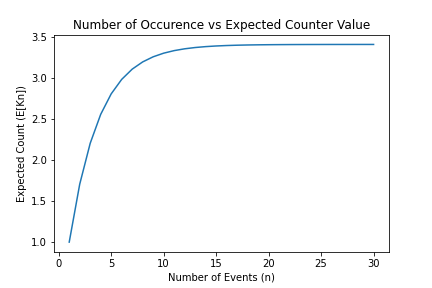
\includegraphics[width=280px, height=200px]{imgs/decreasing.png}
			\end{center}		
		\end{figure}
	
		As it can be clearly observed from Fig. (\ref{figure:decreasingProb}), the expected counter values as $n\to \infty$ becomes constant for $n > 10$. Hence, we can determine the upper-bound for the expected counter values by evaluating the limit of the sum function of Equation (\ref{equation:3}) as $n \to \infty$.
		\begin{align*}
			\intertext{Let $\phi(k_n) \ge \mathbb{E}[k_n], \forall n$ be an upper-bound for $\mathbb{E}[k_n]$}
			\phi(k_n)=&\lim_{n\to \infty}\dfrac{2^{(1-\frac{n}{2})}-2}{\sqrt{2}-2} \\
			=&\lim_{n\to \infty}\dfrac{2^{(1-\frac{n}{2})}-2}{\sqrt{2}-2}\cdot \dfrac{\sqrt{2}+2}{\sqrt{2}+2}\\
			=&\lim_{n\to \infty} 2^{\frac{1}{2}}+2-2^{\frac{1-n}{2}}-2^{\frac{2-n}{2}} \\
			\therefore \phi(k_n)=&\sqrt{2}+2 \\
			\approx & 3.14142
		\end{align*}
		Hence, after about $10$ events, the expected counter values for all future occurrences tend to approach $\sqrt{2}+2$.
	
	\section{Auxiliary Functions}
	
		
	\bibliography{references} % use a field named url or \url{} for URLs
	% Note: the \bibliographystyle is set automatically
	
\end{document}
